%----------------------------------------------------------------------------------------
%    PACKAGES AND THEMES
%----------------------------------------------------------------------------------------

\documentclass[aspectratio=169,xcolor=dvipsnames]{beamer}
\usetheme{SimplePlus}

\usepackage{hyperref}
\usepackage{graphicx} % Allows including images
\usepackage{booktabs} % Allows the use of \toprule, \midrule and \bottomrule in tables

%----------------------------------------------------------------------------------------
%    TITLE PAGE
%----------------------------------------------------------------------------------------

\title{Pattern Recognition \\ \& Machine Learning}
\subtitle{Project's Presentation}

\author{Aristeidis Daskalopoulos (10640), Georgios Rousomanis (10703)}

\institute
{
    Aristotle University of Thessaloniki\\
    Department of Electrical and Computer Engineering
}
\date{\today} % Date, can be changed to a custom date

%----------------------------------------------------------------------------------------
%    PRESENTATION SLIDES
%----------------------------------------------------------------------------------------

\begin{document}

\begin{frame}
    % Print the title page as the first slide
    \titlepage
\end{frame}



\begin{frame}{Part A - Intro}

    In this part, we address a \textbf{binary classification problem} where the goal is to classify samples into one of two classes: $\omega_1$ or $\omega_2$, based on \textit{a single feature} $x$ (a feature vector of dimensionality one).

    \vspace{5pt}
    
    To achieve this, we use the probability density function (PDF) of the feature $x$, which follows - for both classes - the distribution described below:
    
    $$ p(x|\theta) = \frac{1}{\pi}\frac{1}{1 + (x - \theta)^2} \quad, $$
    
    where $\theta$ is an unknown parameter which has to be defined for each one of the classes separately. \textit{This PDF is the probability distribution of the Cauchy distribution for $\gamma = 1$.} 

    \vspace{5pt}

    \begin{center}
        To solve this decision problem, we will implement a Generative Probabilistic Model, following the steps described in the subsequent slides.
    \end{center}
    
\end{frame}

% -----------------------------------------------

\begin{frame}{1. Maximum Likelihood Estimation (MLE)}

    Our first goal is to estimate the parameters $\hat{\theta}_1$ and $\hat{\theta}_2$ using the Maximum Likelihood (ML) method. To do this, we aim to maximize the log-likelihood function with respect to $\theta_j$, for $j = 1, 2$; $\theta_1$ is the parameter of the first class, and $\theta_2$ refers to class $\omega_2$.

    \vspace{5pt}
    
    Assuming that the samples $D_j$ of the class $\omega_j$, for $j = 1, 2$, are \textit{independent and identically distributed (i.i.d.)}, meaning they have been drawn independently from the same distribution $p(x | \theta_j, \omega_j)$, the PDF for the samples can be expressed as:

    $$ p(D_j | \theta_j) = \prod_{i=1}^{N_j} p(x_i | \theta_j)\quad.$$ 

    We prefer to work with the log-likelihood function, because it simplifies the process - as it converts multiplication into addition, which is \textit{less} error-sensitive in terms of computational arithmetic errors (and in terms of calculating derivates).
    
\end{frame}

% -----------------------------------------------

\begin{frame}{1. MLE - log-likelihood $l(\theta_j)$}

    The log-likelihood of our problem is:
    
    $$ l(\theta_j) = \log p(D_j | \theta_j) = \sum_{i=1}^{N_j} \log p(x_i | \theta_j), \quad j = 1, 2 \quad \Rightarrow$$
    
    $$ l(\theta_j) = - N_j \cdot \log \pi - \sum_{i=1}^{N_j} \log (1 + (x_i - \theta_j)^2), \quad j = 1, 2 \quad,$$

    with which we can estimate the $\hat{\theta}_j$ for each class. This estimate, $\hat{\theta}_j$, is by definition the value of $\theta_j$ that maximizes the likelihood/log-likelihood. 

    \vspace{5pt}
    
    In our case the term $- N_j \cdot \log \pi$ is constant, so we practically just need to \textit{minimize} the positive term $\sum_{i=1}^{N_j} \log (1 + (x_i - \theta_j)^2)$. \textit{It is important to keep in mind that the specific $l(\theta)$ is a negative function.}
    
\end{frame}

% -----------------------------------------------

\begin{frame}{1. MLE - log-likelihood $l(\theta_j)$ - Find $\hat{\theta}_j$}

    One approach to solving this problem is to calculate the derivatives and solve the following equations, where the solution gives the estimate $\hat{\theta}_j$ for each class:

    $$ \frac{d}{d\theta_j} l(\theta_j) = 0 \Rightarrow \frac{d}{d\theta_j} \left(- N_j \cdot \log \pi - \sum_{i=1}^{N_j} \log (1 + (x_i - \theta_j)^2)\right) = 0 \Rightarrow  \sum_{i=1}^{N_j} \frac{-2 \cdot (x_i - \theta_j)}{1 + (x_i - \theta_j)^2} = 0.$$

    \begin{center}
        \textit{For all the $\hat{\theta}_j$ that solve the above equation we should choose the one that gives the largest (max) value to the $l(\theta_j)$.}
    \end{center}

    Given $l(\theta_j)$, its derivative can be computed efficiently (e.g., using a library like SymPy) to solve the equation and obtain the estimate $\hat{\theta}_j$. However, by plotting $l(\theta_j)$ as requested, we inherently \textit{calculate the values of the log-likelihood function across multiple points}. Consequently, selecting the value of $\theta$ that maximizes $l(\theta)$ provides the same solution, thereby \textbf{avoiding} the need for the derivative-based approach.
    
    
\end{frame}

% -----------------------------------------------

\begin{frame}{1. Maximum Likelihood Estimation (Results)}

    We execute the \texttt{fit} method for each dataset, $D_j$, to determine the optimal Maximum Likelihood estimations, $\hat{\theta}_j$. Additionally, we plot the log-likelihood function:

    \vspace{-10pt}

    $$ l(\theta) = \log P(D_j | \theta), \quad \text{for} \; j = 1, 2, $$
    
    and highlight the point where the likelihood reaches its maximum.

    \begin{table}
        \centering
        \begin{tabular}{cc}
            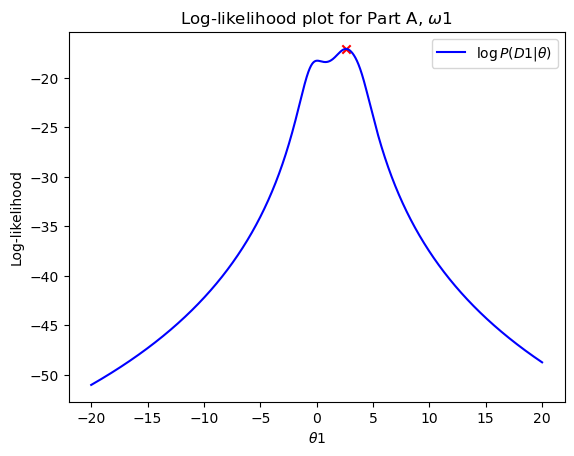
\includegraphics[width=0.4\linewidth]{out/plot1_MLE1.png} &
            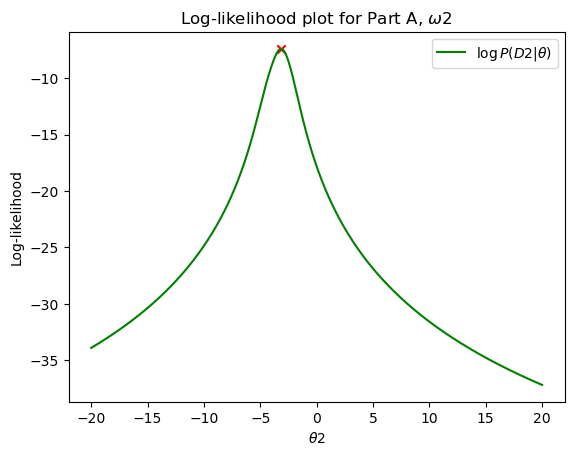
\includegraphics[width=0.4\linewidth]{out/plot2_MLE2.png} \\
        \end{tabular}
        \label{tab:1}
    \end{table}

    \vspace{-10pt}

    Results: $\theta_1$ ML estimation (no stress): 2.598, $\theta_2$ ML estimation (intense stress): -3.158
    
\end{frame}

% -----------------------------------------------

\begin{frame}{2. Bayes Decision Rule}

    Using the Bayes Decision Rule, we classify to $\omega_1$ based on the following condition:
    
    $$ P(\omega_1 | x) > P(\omega_2 | x) \quad, $$
    
    which can be rewritten using the \textit{Bayes formula} as:
    
    $$ \frac{p(x|\omega_1) P(\omega_1)}{p(x)} > \frac{p(x|\omega_2) P(\omega_2)}{p(x)} \Rightarrow \log p(x|\omega_1) + \log P(\omega_1) > \log p(x|\omega_2) + \log P(\omega_2) \quad. $$
    
    \textit{Here, the class-conditional densities $p(x|\omega_1, \theta_1)$ and $p(x|\omega_2, \theta_2)$ have been fully defined using Maximum Likelihood (ML) estimation, for the parameters $\theta_1 = \hat{\theta}_1$ and $\theta_2 = \hat{\theta}_2$ respectively.} So, for each class we have that:
    
    $$ p(x|\omega_j) = \frac{1}{\pi}\frac{1}{1 + (x - \hat{\theta}_j)^2}, \quad P(\omega_j) = \frac{|D_j|}{|D_1| + |D_2|}, $$
    
    where $|D_j|$ is the total number of elements, $N_j$, that this dataset has.
    
\end{frame}

% -----------------------------------------------

\begin{frame}{2. Bayes Decision Rule - Discriminant Function $g(x)$}

    We define the following discriminant function:

    $$ g(x) = \log p(x|\omega_1) - \log p(x|\omega_2) + \log P(\omega_1) - \log P(\omega_2) \quad, $$
    
    and based on the previous inequity we infer that using this discriminant function:

    \begin{itemize}
        \item If $g(x) > 0$, the sample with feature $x$ is classified into class $\omega_1$.
        \item Otherwise, it is classified into class $\omega_2$.

    \end{itemize}
    
    The above \textbf{rule} implies that we theoretically expect the discriminant function $g(x)$ to be greater than zero when a sample from the $D_1$ set (class $\omega_1$) is provided. 

    \vspace{5pt}
    
    Based on this rule, the feature space - represented by the real number line $\mathbb{R}$ - is divided into two distinct regions: $\mathbb{R}_1$ and $\mathbb{R}_2$. To complete the theoretical analysis of this section, these regions must be defined by determining their boundaries, which can be found by solving $g(x) = 0$
    
\end{frame}

% -----------------------------------------------

\begin{frame}{2. Bayes Decision Rule - $g(x) = 0$}

    \vspace{-15pt}

    $$ \log(\frac{1}{\pi}\frac{1}{1 + (x - \hat{\theta}_1)^2}) - \log(\frac{1}{\pi}\frac{1}{1 + (x - \hat{\theta}_2)^2}) + \log(\frac{|D_1|}{|D_1| + |D_2|}) - \log(\frac{|D_2|}{|D_1| + |D_2|}) = 0 \quad \Rightarrow$$

    \vspace{-5pt}

    $$ -\log(1 + (x - \hat{\theta}_1)^2) + \log(1 + (x - \hat{\theta}_2)^2) + \log(\frac{|D_1|}{|D_2|}) = 0, \quad Let\ r = \frac{|D_1|}{|D_2|} \quad \Rightarrow$$

    \vspace{-5pt}
    
    $$ \log(\frac{1 + (x - \hat{\theta}_2)^2}{1 + (x - \hat{\theta}_1)^2}) = -\log(r) \quad \Rightarrow \quad \frac{1 + (x - \hat{\theta}_2)^2}{1 + (x - \hat{\theta}_1)^2} = \frac{1}{r} \quad \Rightarrow$$

    \vspace{-5pt}
    
    $$ r(1 + (x - \hat{\theta}_2)^2) = 1 + (x - \hat{\theta}_1)^2 \quad \Rightarrow \quad (r-1)x^2 - 2(r\hat{\theta}_2 - \hat{\theta}_1)x + (r\hat{\theta}_2^2 + r - \hat{\theta}_1^2 - 1) = 0 $$
    
    The solutions to this quadratic equation define the decision boundary points. These points separate regions $\mathbb{R}_1$ and $\mathbb{R}_2$ in the feature space. 
    
    If the equation above has two real solutions, $x_a$ and $x_b$, then one of the regions, $\mathbb{R}_j$, will be an interval spanning $(-\infty, x_a) \cup (x_b, +\infty)$, while the other will correspond to the interval $[x_a, x_b]$. We will specify these intervals after estimating the values of $\hat{\theta}_j$.
    
\end{frame}

% -----------------------------------------------

\begin{frame}{2. Bayes Decision Rule (Results)}

    \vspace{-5pt}

    Having determined the values of $\hat{\theta}_1$ and $\hat{\theta}_2$ based on the datasets $D_1\ \text{and}\ D_2$ \textit{and} explained the classification rule, the next step is to evaluate whether we can correctly classify the training dataset/examples. This serves as a preliminary test to assess the model's ability to separate the classes using the learned parameters.

    \vspace{-5pt}

    \begin{figure}
        \centering
        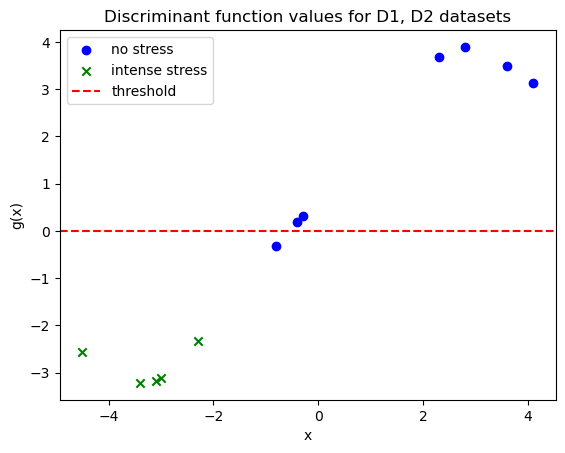
\includegraphics[width=0.5\linewidth]{out/plot3_discriminantValues.png}
        \label{fig:1}
    \end{figure}
    
\end{frame}

% -----------------------------------------------

\begin{frame}{2. Bayes Decision Rule (Results)}

    From the previous plot, we observe only one misclassification, where a sample that should have been classified as "no stress" was incorrectly predicted as "intense stress." Additionally, it is evident that some "no stress" values are near the threshold.  

    \vspace{5pt}

    We should now implement a validation method to ensure that the classifier can correctly classify samples it has \textbf{never seen before}. It is important to note that, due to the very limited number of training samples, splitting $D_1 \cup D_2$ into training and validation sets may not yield reliable results. To address this, we will use \textit{Leave-One-Out Cross-Validation} (LOOCV) to evaluate the accuracy, precision, and recall of our model. This approach ensures that every sample is used both for training and as a validation point at least once. 
    
    By employing LOOCV, we can verify that our approach is truly learning the underlying patterns (and not merely memorizing the training set). Additionally, this provides a consistent metric for \textit{comparison with the results obtained in Part B.}
    
\end{frame}

% -----------------------------------------------

\begin{frame}{2. Bayes Decision Rule (LOOCV)}

    The classifier performance metrics are as follows:
    \begin{itemize}
        \item $\omega_1$: ``relaxed'' label (positive)
        \item $\omega_2$: ``stressed'' label (negative)
    \end{itemize}
    
    \begin{enumerate}
        \item \textbf{Accuracy}: $0.833$  
        Overall correctness of the classifier.
    
        \item \textbf{Precision}: $1.0$  
        All predicted ``relaxed'' samples are correct.
    
        \item \textbf{Recall}: $0.714$  
        71.43\% of true ``relaxed'' samples were detected.
    
        \item \textbf{F1 Score}: $0.833$  
        Balanced performance measure (precision and recall).
    \end{enumerate}
    
    \textit{Note}: In the previous analysis, without domain knowledge of the game, we focused on the "relaxed/no stress" label. This decision was based on our observation that the model tends to make more errors when predicting this label. Despite these challenges, the overall accuracy remains acceptable, considering the very limited number of examples available in our dataset.

    
\end{frame}

% -----------------------------------------------

\begin{frame}{2. Bayes Decision Rule (Decision Regions)}

    \textbf{Lastly}, based on the previously evaluated $\hat{\theta}_j$ results, we can \textit{solve the equation}: $g(x) = 0$ and determine the two regions, $\mathbb{R}_1$ and $\mathbb{R}_2$, in the feature space. By determining these regions, we would have \textbf{fully explained the classification rule}, whose accuracy on the dataset has \textit{already} been measured using LOOCV.

    We have found that $\hat{\theta}_1 \simeq 2.6$ and $\hat{\theta}_2 \simeq -3.16$. To solve the quadratic equation:

    \vspace{-10pt}
    
    $$ (r-1)x^2 - 2(r\hat{\theta}_2 - \hat{\theta}_1)x + (r\hat{\theta}_2^2 + r - \hat{\theta}_1^2 - 1) = 0, $$

    \vspace{-5pt}
    
    where $r = \frac{7}{5}$, we can apply the quadratic formula and get the roots:

    \vspace{-15pt}
    
    $$ x_a \approx −34.57, \quad x_b \approx −0.55.$$

    \vspace{-7pt}
    
    These values define the boundaries of the regions $\mathbb{R}_1$ and $\mathbb{R}_2$ in the feature space and we can also visualize/validate them by evaluating the $g(x)$ sign with specific values:

    \vspace{-5pt}

    \begin{figure}
        \centering
        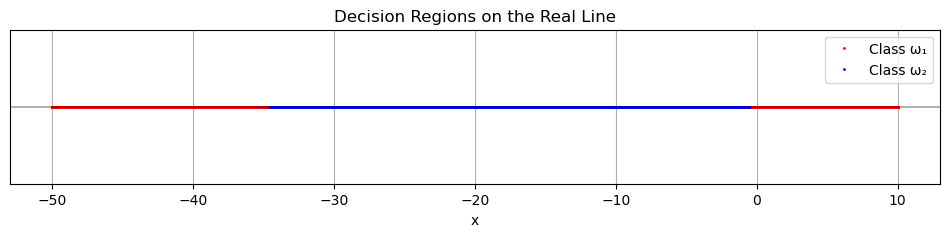
\includegraphics[width=0.7\linewidth]{out/plot4_DecisionRegions.png}
        \label{fig:1}
    \end{figure}

\end{frame}

% -----------------------------------------------

\begin{frame}{Part B - Intro}

    In the earlier section, we worked with a limited dataset to classify samples using the \textit{Maximum Likelihood} estimation for the parameter $\theta$ for each class. The classification was performed based on the feature "vector" (has a dimensionality of one) $x \in \mathbb{R}$. 

    Now we need to:

    \vspace{-5pt}

    \begin{itemize}
        \item Extend the approach by incorporating the \textit{prior knowledge} of the probability distribution $p(\theta)$ and use this prior knowledge to make a refined estimate of the \textit{posterior} distribution of $\theta$.
        \item Expect the posterior distribution to be \textbf{sharply concentrated around the true value} of $\theta$, improving accuracy and reliability.
        \item Use the posterior distribution to provide a more precise and informed estimate of $\theta$.
    \end{itemize}
    
    The \textit{prior PDF} of $\theta$ is defined as:  

    $$ p(\theta_j) = \frac{1}{10\pi} \frac{1}{1 + (\theta_j / 10)^2}, \quad j = 1, 2 \quad.$$

\end{frame}

% -----------------------------------------------

\begin{frame}{1. Bayesian Estimation: Posterior PDF of $\theta$}

    Given the dataset $D_j$ for class $\omega_j$, the \textbf{likelihood function} is computed as:

    \vspace{-10pt}

    $$ p(D_j|\theta_j) = \prod_{n=1}^{N_j} p(x_n|\theta_j), \quad j = 1, 2 \quad, $$
    
    where, $N_j$ denotes the number of samples in $D_j$, and $p(x_n|\theta_j)$ represents the likelihood of observing the feature $x_n$ given the parameter $\theta_j$.
     
    Using Bayes' theorem, the \alert{posterior PDF} of $\theta$ is given by:  

    \vspace{-10pt}
    
    $$ p(\theta_j|D_j) = \frac{p(D_j|\theta_j) p(\theta_j)}{\int p(D_j|\theta_j) p(\theta_j) \, d\theta_j}, \quad j = 1, 2 \quad. $$

    To determine the posterior PDF of $\theta$, we execute the \texttt{posterior\_theta\_pdf} method for each dataset $D_j$. We also evaluate the \textit{Maximum A Posteriori} (MAP) estimates of $\theta_1 \& \theta_2$. 

    \vspace{5pt}

    We expect these estimates to closely match (or \textit{at least be near to}) the results obtained from the MLE of $\theta_j$. Additionally, we compute the prior PDF of $\theta$, using the \texttt{prior\_theta\_pdf} method, and plot all the results on the same diagram for comparison.


\end{frame}

% -----------------------------------------------

\begin{frame}{Bayesian Estimation: Posterior PDF of $\theta$ (Results)}

    \begin{itemize}
        \item MAP estimate of $\theta_1$ (no stress):       2.603
        \item MAP estimate of $\theta_2$ (intense stress): -3.163
    \end{itemize}

    \begin{figure}
        \centering
        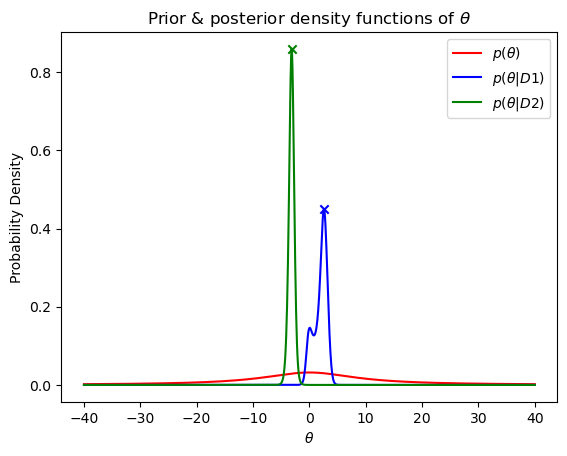
\includegraphics[width=0.5\linewidth]{out/plot5_PriorAndPosteriorPDFofTheta.png}
        \label{fig:1}
    \end{figure}


\end{frame}

% -----------------------------------------------

\begin{frame}{Bayesian Estimation: Posterior PDF of $\theta$ (Results)}

    Conclusions:
    \begin{itemize}
        \item The posterior density functions $p(\theta | D_j)$ are sharply concentrated around their respective \textit{MAP estimates}, which closely align with the \textit{Maximum Likelihood (ML) estimates}. This indicates that the posterior distributions provide confident estimates of $\theta$, as \textit{informed by the datasets $D_j$}.

        \item In contrast, the prior $p(\theta)$ is a much wider distribution, offering less confidence in its estimates when considered alone. As a result, \textbf{the posterior is primarily informed} by the data in the datasets $D_j$, with respect to the prior $p(\theta)$ which also influences the final results.

        \item To assess whether the knowledge of the prior $p(\theta)$ has a significant impact, we will once again perform LOOCV for the new classifier and evaluate the resulting performance metrics.
        
    \end{itemize}

\end{frame}

% -----------------------------------------------

\begin{frame}{2. Bayesian Estimation: Decision}

    Using the \textit{Bayesian Estimation (BE)}, we classify to $\omega_1$ based on the following condition:

    \vspace{-5pt}

    $$ p(\omega_1 | x, D_1) > p(\omega_2 | x, D_2) $$
    
    which also can be rewritten using the \textit{Bayes formula} as:
    
    $$ 
    \frac{p(x | D_1) P(\omega_1)}{p(x | D_1) P(\omega_1) + p(x | D_2) P(\omega_2)} > 
    \frac{p(x | D_2) P(\omega_2)}{p(x | D_1) P(\omega_1) + p(x | D_2) P(\omega_2)} \Rightarrow
    $$
    
    $$ \log p(x | D_1) + \log P(\omega_1) > \log p(x | D_2) + \log P(\omega_2) \quad. $$

    \vspace{5pt}
    
    By selecting the following discriminant function:

    \vspace{-10pt}
    
    $$ h(x) = \log p(x | D_1) - \log p(x | D_2) + \log P(\omega_1) - \log P(\omega_2) \quad, $$
    
    we once again classify an element/sample with feature value $x$ into class $\omega_1$ if $h(x) > 0$, and into class $\omega_2$ otherwise. \textit{This same classification \textbf{rule} was applied in Part A}. However, this time we need to determine the \alert{class conditional density $p(x | D_j)$}.


\end{frame}

% -----------------------------------------------

\begin{frame}{2. Bayesian Estimation: Decision - $p(x | D_j)$}

    We have already demonstrated how to compute the posterior density $p(\theta_j | D_j)$. Using this, along with the feature PDF $p(x | \theta_j)$, we can evaluate the \textit{marginal density} $p(x | D_j)$ by integrating the joint density $p(x, \theta | D_j)$ over $\theta$:

    \vspace{-5pt}

    $$ p(x | D_j) = \int p(x, \theta | D_j) \, d\theta. $$
    
    By applying the product rule and because the selection of
    $x$ and $D_j$ are done \textit{independently}, this equation can be rewritten as:

    \vspace{-5pt}
    
    $$ p(x | D_j) = \int_{-\infty}^{+\infty} p(x | \theta) p(\theta | D_j) \, d\theta. $$
    
    The above integral can be easily computed using the \textbf{trapezoidal rule}. Instead of letting $\theta$ range from $-\infty$ to $+\infty$, we can limit the integration to two sufficiently large bounds. These bounds are chosen to \textit{cover all the significant non-zero areas} of the distributions. For very large or very small values of $\theta$, the product of the distributions becomes nearly zero. As a result, these values have negligible effect on the overall computation.

\end{frame}

% -----------------------------------------------

\begin{frame}{2. Bayesian Estimation: Decision (Results)}

    \begin{columns}[c] % The "c" option specifies centered vertical alignment while the "t" option is used for top vertical alignment

        \column{.45\textwidth} % Left column and width
        \begin{figure}
            \centering
            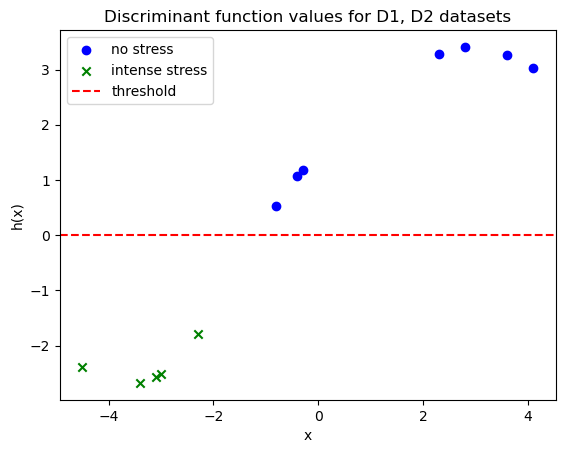
\includegraphics[width=1.15\linewidth]{out/plot6_discriminantValuesPartB.png}
            \label{fig:1}
        \end{figure}
        

        \column{.45\textwidth} % Right column and width
        Before performing LOOCV to compare this classifier's performance metrics with the one at part A - \textit{to gain a clearer understanding of the superiority of the current classifier (B) over the previous one}, we first test the model's ability to correctly classify the training datasets $D_j$. This serves as a preliminary evaluation to verify whether the model can effectively distinguish between the classes, using the learned parameters.

    \end{columns}

\end{frame}

% -----------------------------------------------

\begin{frame}{2. Bayesian Estimation: Decision (Conclusions)}

    It is evident - based on the previous plot - that BE gives us better results than MLE, because this time $h(x) > 0$ for all the $D_1$ dataset, with no values of $h(x)$ "too close" to the threshold (they are further than the previous classifier). This is beacause it takes into account the prior distribution of the $\theta$ parameter, leading to better solutions.

    \vspace{5pt}

    To confirm the validity of this finding, we validate our model using the same datasets $D_j$, applying the LOOCV method \textit{as done in Part A}. This allows us to assess the model's ability to predict unseen samples. 

    \begin{block}{Performance Metrics For Part B Classifier}
        Accuracy:  0.9167 |
        Precision: 1.0 |
        Recall:    0.8571 |
        F1 Score:  0.9231
    \end{block}

    The improved results demonstrate the \textbf{advantage of incorporating the prior $p(\theta)$ into the model}. The higher accuracy and F1 score indicate that the classifier is better at distinguishing between classes, while we still have precision 1.0. The increase in recall (from 71.43\%) suggests that the model is capturing  $\approx20\%$ more true positives compared to the previous approach, leading to a \textit{more reliable classification}.

\end{frame}

%------------------------------------------------

\begin{frame}{Bullet Points}
    \begin{itemize}
        \item Lorem ipsum dolor sit amet, consectetur adipiscing elit
        \item Aliquam blandit faucibus nisi, sit amet dapibus enim tempus eu
        \item Nulla commodo, erat quis gravida posuere, elit lacus lobortis est, quis porttitor odio mauris at libero
        \item Nam cursus est eget velit posuere pellentesque
        \item Vestibulum faucibus velit a augue condimentum quis convallis nulla gravida
    \end{itemize}
\end{frame}

%------------------------------------------------

\begin{frame}{Blocks of Highlighted Text}
    In this slide, some important text will be \alert{highlighted} because it's important. Please, don't abuse it.

    \begin{block}{Block}
        Sample text
    \end{block}

    \begin{alertblock}{Alertblock}
        Sample text in red box
    \end{alertblock}

    \begin{examples}
        Sample text in green box. The title of the block is ``Examples".
    \end{examples}
\end{frame}

%------------------------------------------------

\begin{frame}{Multiple Columns}
    \begin{columns}[c] % The "c" option specifies centered vertical alignment while the "t" option is used for top vertical alignment

        \column{.45\textwidth} % Left column and width
        \textbf{Heading}
        \begin{enumerate}
            \item Statement
            \item Explanation
            \item Example
        \end{enumerate}

        \column{.45\textwidth} % Right column and width
        Lorem ipsum dolor sit amet, consectetur adipiscing elit. Integer lectus nisl, ultricies in feugiat rutrum, porttitor sit amet augue. Aliquam ut tortor mauris. Sed volutpat ante purus, quis accumsan dolor.

    \end{columns}
\end{frame}

%------------------------------------------------

\begin{frame}{Table}
    \begin{table}
        \begin{tabular}{l l l}
            \toprule
            \textbf{Treatments} & \textbf{Response 1} & \textbf{Response 2} \\
            \midrule
            Treatment 1         & 0.0003262           & 0.562               \\
            Treatment 2         & 0.0015681           & 0.910               \\
            Treatment 3         & 0.0009271           & 0.296               \\
            \bottomrule
        \end{tabular}
        \caption{Table caption}
    \end{table}
\end{frame}

%------------------------------------------------

\begin{frame}{Theorem}
    \begin{theorem}[Mass--energy equivalence]
        $E = mc^2$
    \end{theorem}
\end{frame}

%------------------------------------------------

\begin{frame}{Figure}
    Uncomment the code on this slide to include your own image from the same directory as the template .TeX file.
    %\begin{figure}
    %\includegraphics[width=0.8\linewidth]{test}
    %\end{figure}
\end{frame}

%------------------------------------------------

\begin{frame}[fragile] % Need to use the fragile option when verbatim is used in the slide
    \frametitle{Citation}
    An example of the \verb|\cite| command to cite within the presentation:\\~

    This statement requires citation \cite{p1}.
\end{frame}

%------------------------------------------------

\begin{frame}{References}

    \begin{table}
        \centering
        \begin{tabular}{cc}
            \includegraphics[width=0.4\linewidth]{example-image} &
            \includegraphics[width=0.4\linewidth]{example-image} \\
        \end{tabular}
        \caption{Example of multiple images.}
        \label{tab:1}
    \end{table}
\end{frame}

%------------------------------------------------

\begin{frame}

    \begin{figure}
        \centering
        \includegraphics[width=0.5\linewidth]{example-image}
        \caption{Example of single image.}
        \label{fig:1}
    \end{figure}

    \Huge{\centerline{\textbf{The End}}}
\end{frame}

%----------------------------------------------------------------------------------------

\end{document}